\documentclass[10pt,answers]{exam}
\usepackage{listings}
\usepackage{pdfsync}

%
%  Created by Mike Helmick on 2006-09-13.
%  Copyright (c) 2006 Mike Helmick. All rights reserved.
%
%

\newif\ifpdf
\ifx\pdfoutput\undefined
\pdffalse % we are not running PDFLaTeX
\else
\pdfoutput=1 % we are running PDFLaTeX
\pdftrue
\fi

\ifpdf
\usepackage{subfigure}
\usepackage[pdftex]{graphicx}
\else
\usepackage{graphicx}
\fi

% exam settings
%\boxedpoints
%\pointsinmargin
\printanswers 
%\noprintanswers

\usepackage{color} 
\definecolor{SolutionColor}{rgb}{0.8,0.9,0.9} 
\shadedsolutions 


%
%  Update these values for running headers
%
\firstpageheader{\bf\Large CSA174}{\bf\Large Quiz 02}{\bf\Large
  2007-10-28 }
\runningheader{CSA 174}{Miami University}{Quiz 02}
\addpoints

\begin{document}

\begin{center} 
  \fbox{\fbox{\parbox{5.5in}{\centering
    CSA174 - Fall 2007 - Quiz 02 \newline
	Miami University \newline
	\newline
 	There are \numquestions\  questions for a total of  \numpoints\ points.
}}}
\end{center} 

% setup standard options for the including code fragments
\lstset{language=Java,numbers=left, numberstyle=\tiny, stepnumber=1, numbersep=5pt, showstringspaces=true}

\vspace{0.1in} 
\hbox to \textwidth{Name:\enspace\hrulefill} 
Please circle your section:
\begin{enumerate}
	\item Section A - 10:00am Lab
	\item Section C - 12:00pm Lab
	\item Section D - 01:00pm Lab
\end{enumerate} 

\begin{center} 
\gradetable[h][questions] 
\end{center}

% Questions start here:
\begin{questions}
	
\section*{Code Analysis}

\question Determine the output from the following statements, write "no output" if there is no output.
\begin{parts}
	\part[3] Determine the output:
\begin{verbatim}
String x = new String("Hello");
System.out.println( x.toLowerCase() );
\end{verbatim}
\begin{solution}[0.75in]
hello
\end{solution}
	
	\part[3] Determine the output:
\begin{verbatim}
String x = new String("Hello");
y = x;
x = "Moose";
System.out.println( x + y );	
\end{verbatim}
\begin{solution}[0.75in]
MooseHello	
\end{solution}

	\part[3] Determine the output:
\begin{verbatim}
String x = "X" + "Y";
if ( x == "XY" ) {
  System.out.println("true");
} else {
  System.out.println("false");
}
\end{verbatim}
\begin{solution}
false	
\end{solution}

\end{parts}

	
\newpage
\section*{Fill in the blank}

\question[20] Identify the terms by filling in the blanks.  Please be as specific and concise as possible, using vocabulary from the book and/or class.

\begin{figure}[h]
    \begin{center}
        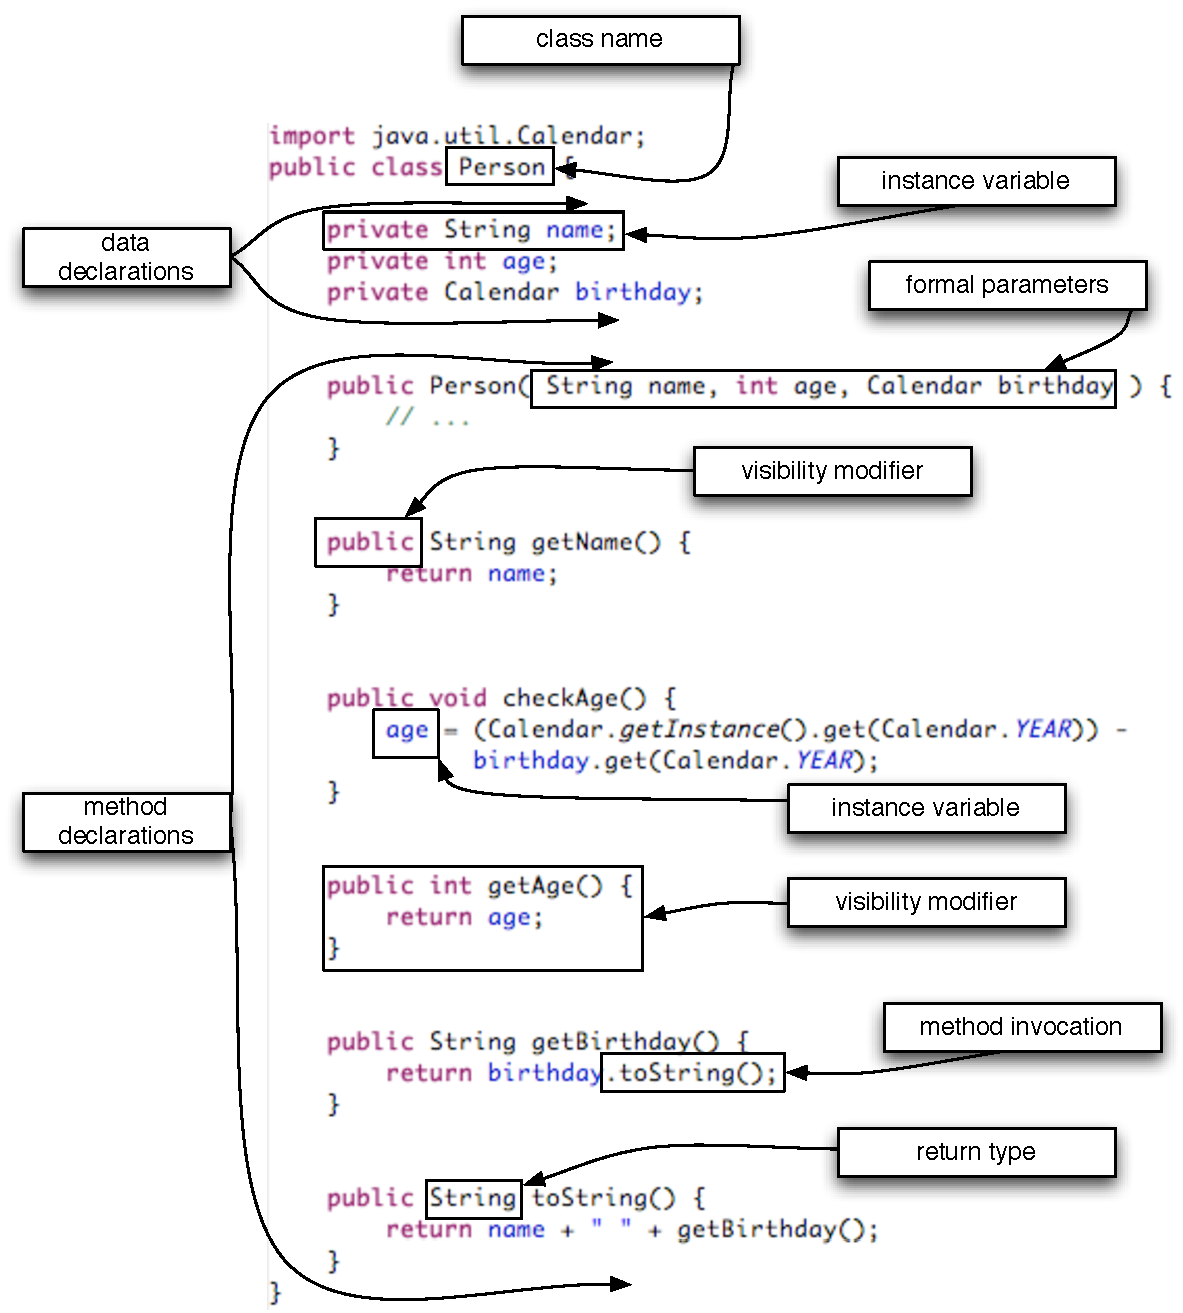
\includegraphics[width=6in]{quiz02diagram_blank}
    \end{center}
\end{figure}

\newpage
\section*{Programming Question}

\question[11] Below is the definition of a class, unfortunately the class is not complete, you are to complete the class as specified in the comments of each method declaration.

\begin{lstlisting}
public class GumballMachine {
	
  // variables for this class
  private int gumballsRemaining;
  private int quartersCollected;
	
  /**
   * Constructor for the gumball machine, takes in a number of gumballs 
   * to initialize the number of gumballs in the machine, the number
   * of quarters collected should be zero
   */
    // START ANSWER
  public GumballMachine(  int gumballs          ) {
    this.gumballsRemaining = gumballs;
	this.quartersCollected = 0;
		
    // END ANSWER
  }
	
  /**
   * Tell the user how many gumballs are remaining in the machine
   */
  public int getGumballsRemaining() {
    // START ANSWER
	return gumballsRemaining;
    // END ANSWER
  }

  /**
   * Return the number of quarters collected
   */
  public int getQuartersCollected() {
    // START ANSWER
	return quartersCollected;
    // END ANSWER
  }
	
  /**
   * Return the amount of money collected (in dollars)
   */
  public double getMoneyCollected() {
    // START ANSWER
	return 0.25 * quartersCollected;
    // END ANSWER	
  }
  /**
   * Purchases a gumball and adds 1 quarter to the machine
   * of course we can only do this if there are gumballs remaining
   */
  public void purchaseGumball() {
    // START ANSWER
	if ( gumballsRemaining > 0 ) {
		gumballsRemaining--;
		quartersCollected++;
	}
    // END ANSWER
  }

  /**
   * Refill the gumball machine with X gumballs
   * During a refil, all quarters are removed from the machine
   */
  public void refillMachine( int x ) {
    // START ANSWER
    gumballsRemaining += x;
    quartersCollected = 0;
    // END ANSWER	
  }	

  /**
   * String representation of the class (your choice)
   */
  public String toString() {
    // START ANSWER
	return String.format("Gumballs left=%d, Quarters in machine=%d",
	                     gumballsRemaining,
	                     quartersCollected );
    // END ANSWER
  }
}
	
\end{lstlisting}

\end{questions}

\end{document}

